\documentclass[10pt,a4paper]{article}
\usepackage{amssymb}
\usepackage{fullpage}
\usepackage{graphicx}
\author{Parker Whaley}
\title{PHYS 351 \#3}
\begin{document}

\maketitle

\section{Q1}
In this question we are asked to consider two states A and B, with the property that B can be reached from A (and incidentally A can be reached from B) along a adiabatic (no heat exchange) series of states modelled by \(P=\alpha V^{-\gamma}\) where \(\gamma=5/3\).  Lets consider the volume changing \(V_{i}\rightarrow V_{f}\) and going from pressure \(P_{i}\rightarrow P_{f}\).  Note that we are in a restricted space since three of these conditions determine the last one, lets take Volume and initial pressure to be given, thus \(\alpha=\frac{P_{i}}{V_{i}^{-5/3}}\) with \(\alpha\) we can now determine the final pressure \(P_{f}=\alpha V_{f}^{-5/3}\).  Now that we have our parameters lets determine the difference in energy of the two states.  \(du=-dw+dq\) where du is change in the state variable, energy, dw is work done by the system and dq is the thermal energy transferred to the system.  We know what the work done by the system is, if a volume expands a little under pressure then it will push on the outside system and do work, or dw=PdV.  Now we need only integrate over a series of states, lets take the states defined by \(P=\alpha V^{-5/3}\) from \(V_{i}\rightarrow V_{f}\). \[w=\int_{V_{i}}^{V_{f}}P(V)dV=\int_{V_{i}}^{V_{f}}\alpha V^{-5/3}dV=[-\frac{3\alpha}{2} V^{-2/3}]\mid_{V_{i}}^{V_{f}}=\frac{3\alpha}{2}[V_{i}^{-2/3}-V_{f}^{-2/3}]\] Since this process was taken along a adiabatic path where there was no heat exchange: \[-\int dw=\int du= \Delta U = \frac{3\alpha}{2}[V_{f}^{-2/3}-V_{i}^{-2/3}]\] Where $\Delta U$ is the energy difference (path invariant) between states A and B.  We may also note that since \(\int dw\) will be positive (we did work on the environment) $\Delta U$ must be negative.\\\\\\

a)  Consider now a different path \(V_{i}\rightarrow V_{f}\) then \(P_{i}\rightarrow P_{f}\).  Let us first ask how much work does the system do.  In general we would integrate dw along both sections of this path however we immediately note that a path that does not change in volume \((dV=0)\) can do no work, thus we need only consider the path \(V_{i}\rightarrow V_{f}\) when computing work done by the system.\[w=\int_{V_{i}}^{V_{f}}P(V)dV=\int_{V_{i}}^{V_{f}}P_{i}dV=P_{i}[V_{f}-V_{i}]\] We also know that energy is conserved and what the energy of the two states are, therefore we can compute q (the net thermal energy into the system).\[\Delta U=-w+q\Rightarrow q=\Delta U+w=\frac{3\alpha}{2}[V_{f}^{-2/3}-V_{i}^{-2/3}]+P_{i}[V_{f}-V_{i}]\]\\\\\\

b)  Consider now the path where volume and pressure are linearly related.  We can model this path as \(P(t)=P_{i}+t(P_{f}-P{i})\) and \(V(t)=V_{i}+t(V_{f}-V_{i})\) note \((V_{f}-V_{i})dt= dV\) where t goes \(0\rightarrow 1\).  Now we can calculate work.\[w=\int_{path}PdV=\int_{0}^{1}(P_{i}+t(P_{f}-P{i}))(V_{f}-V_{i})dt=(V_{f}-V_{i})(P_{i}t+t^2(P_{f}-P_{i})/2)\mid_{0}^{1}=(V_{f}-V_{i})(P_{i}/2+P_{f}/2)\]As in the previous section we can easily calculate q (the net thermal energy into the system)\[\Delta U=-w+q\Rightarrow q=\Delta U+w=\frac{3\alpha}{2}[V_{f}^{-2/3}-V_{i}^{-2/3}]+(V_{f}-V_{i})(P_{i}/2+P_{f}/2)\]\\\\\\







c)  Consider now a different path \(P_{i}\rightarrow P_{f}\) then \(V_{i}\rightarrow V_{f}\).  This proceeds in the same fashion as part a.  Since the same argument applies to the constant volume section we can immediately proceed to:\[w=\int_{V_{i}}^{V_{f}}P(V)dV=\int_{V_{i}}^{V_{f}}P_{f}dV=P_{f}[V_{f}-V_{i}]\]And calculating q:\[\Delta U=-w+q\Rightarrow q=\Delta U+w=\frac{3\alpha}{2}[V_{f}^{-2/3}-V_{i}^{-2/3}]+P_{f}[V_{f}-V_{i}]\]\\\\\\

\subsection{Q2}
We are asked to consider the van der Waals equation of state for imperfect gas:\[P=\frac{RT}{v-b}-\frac{a}{v^2}\]Consider hexane where \(a=2.50374\frac{Jm^3}{mol^2}\)  \(b=1.735E-4\frac{m^3}{mol}\) at a temperature of \(T=300K\).  Below are some plots of the pressure as a function of molar volume.  In a ideal gas we would expect the pressure and volume to be inversely related, this is not at all what happens in this model.

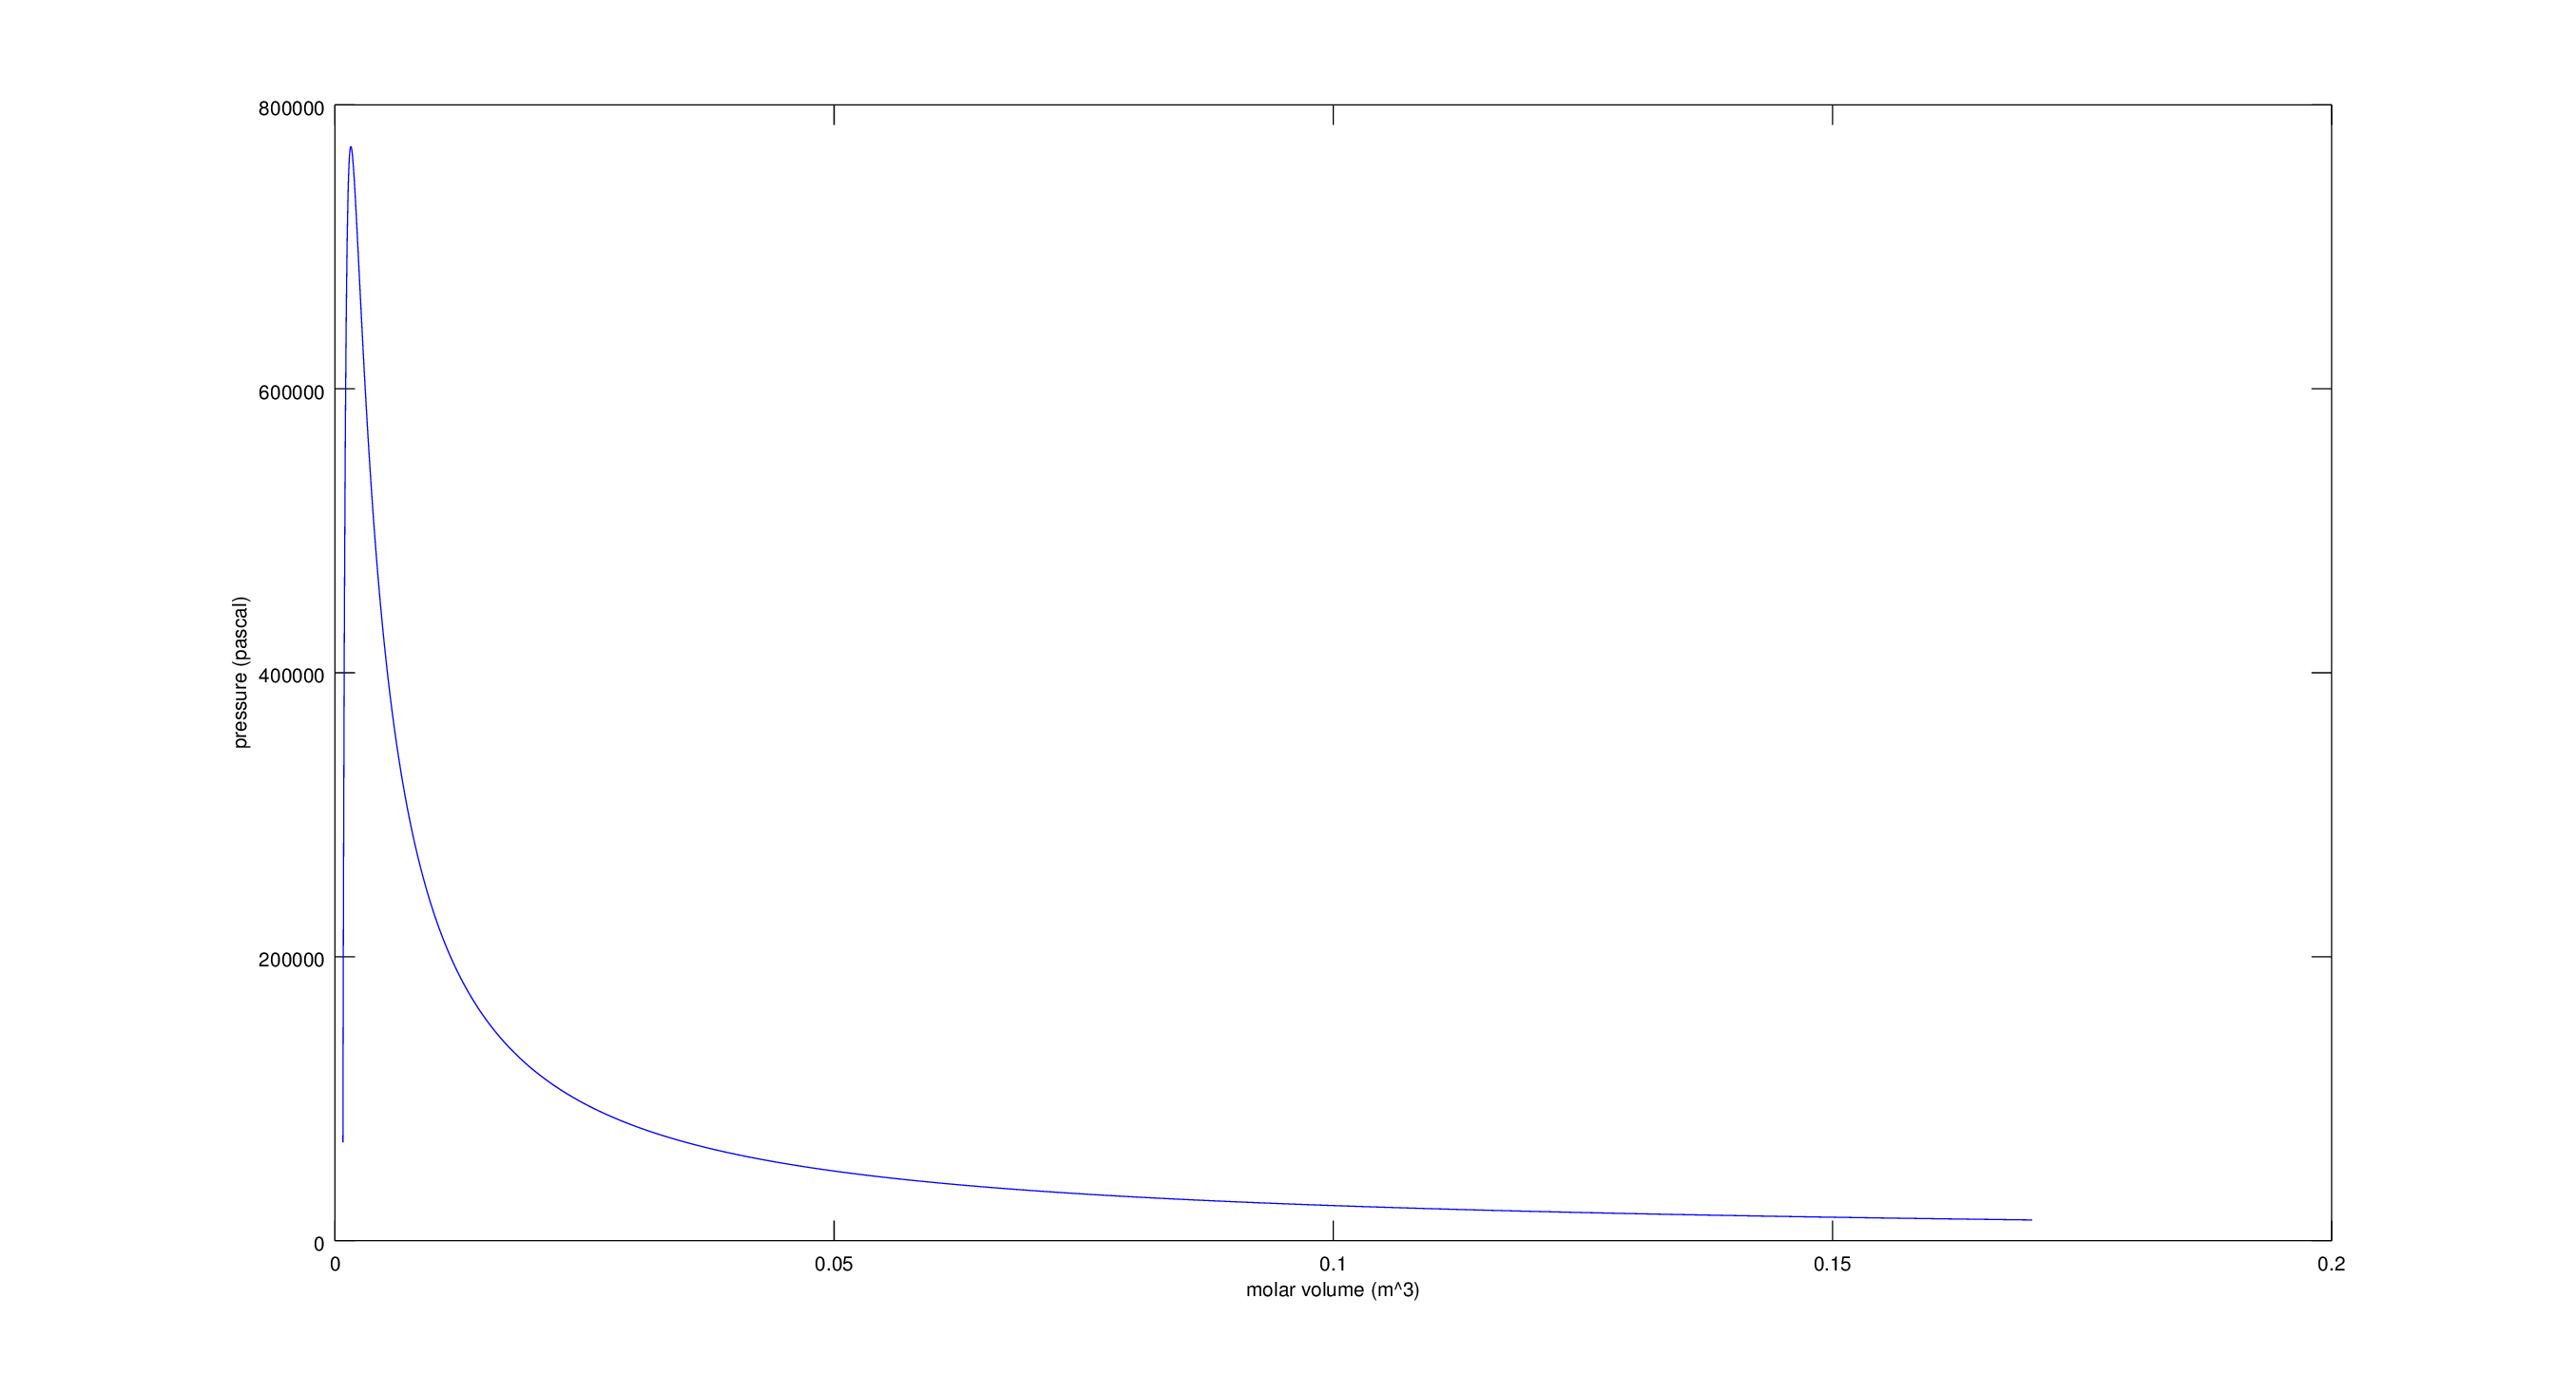
\includegraphics[scale=.35]{one}

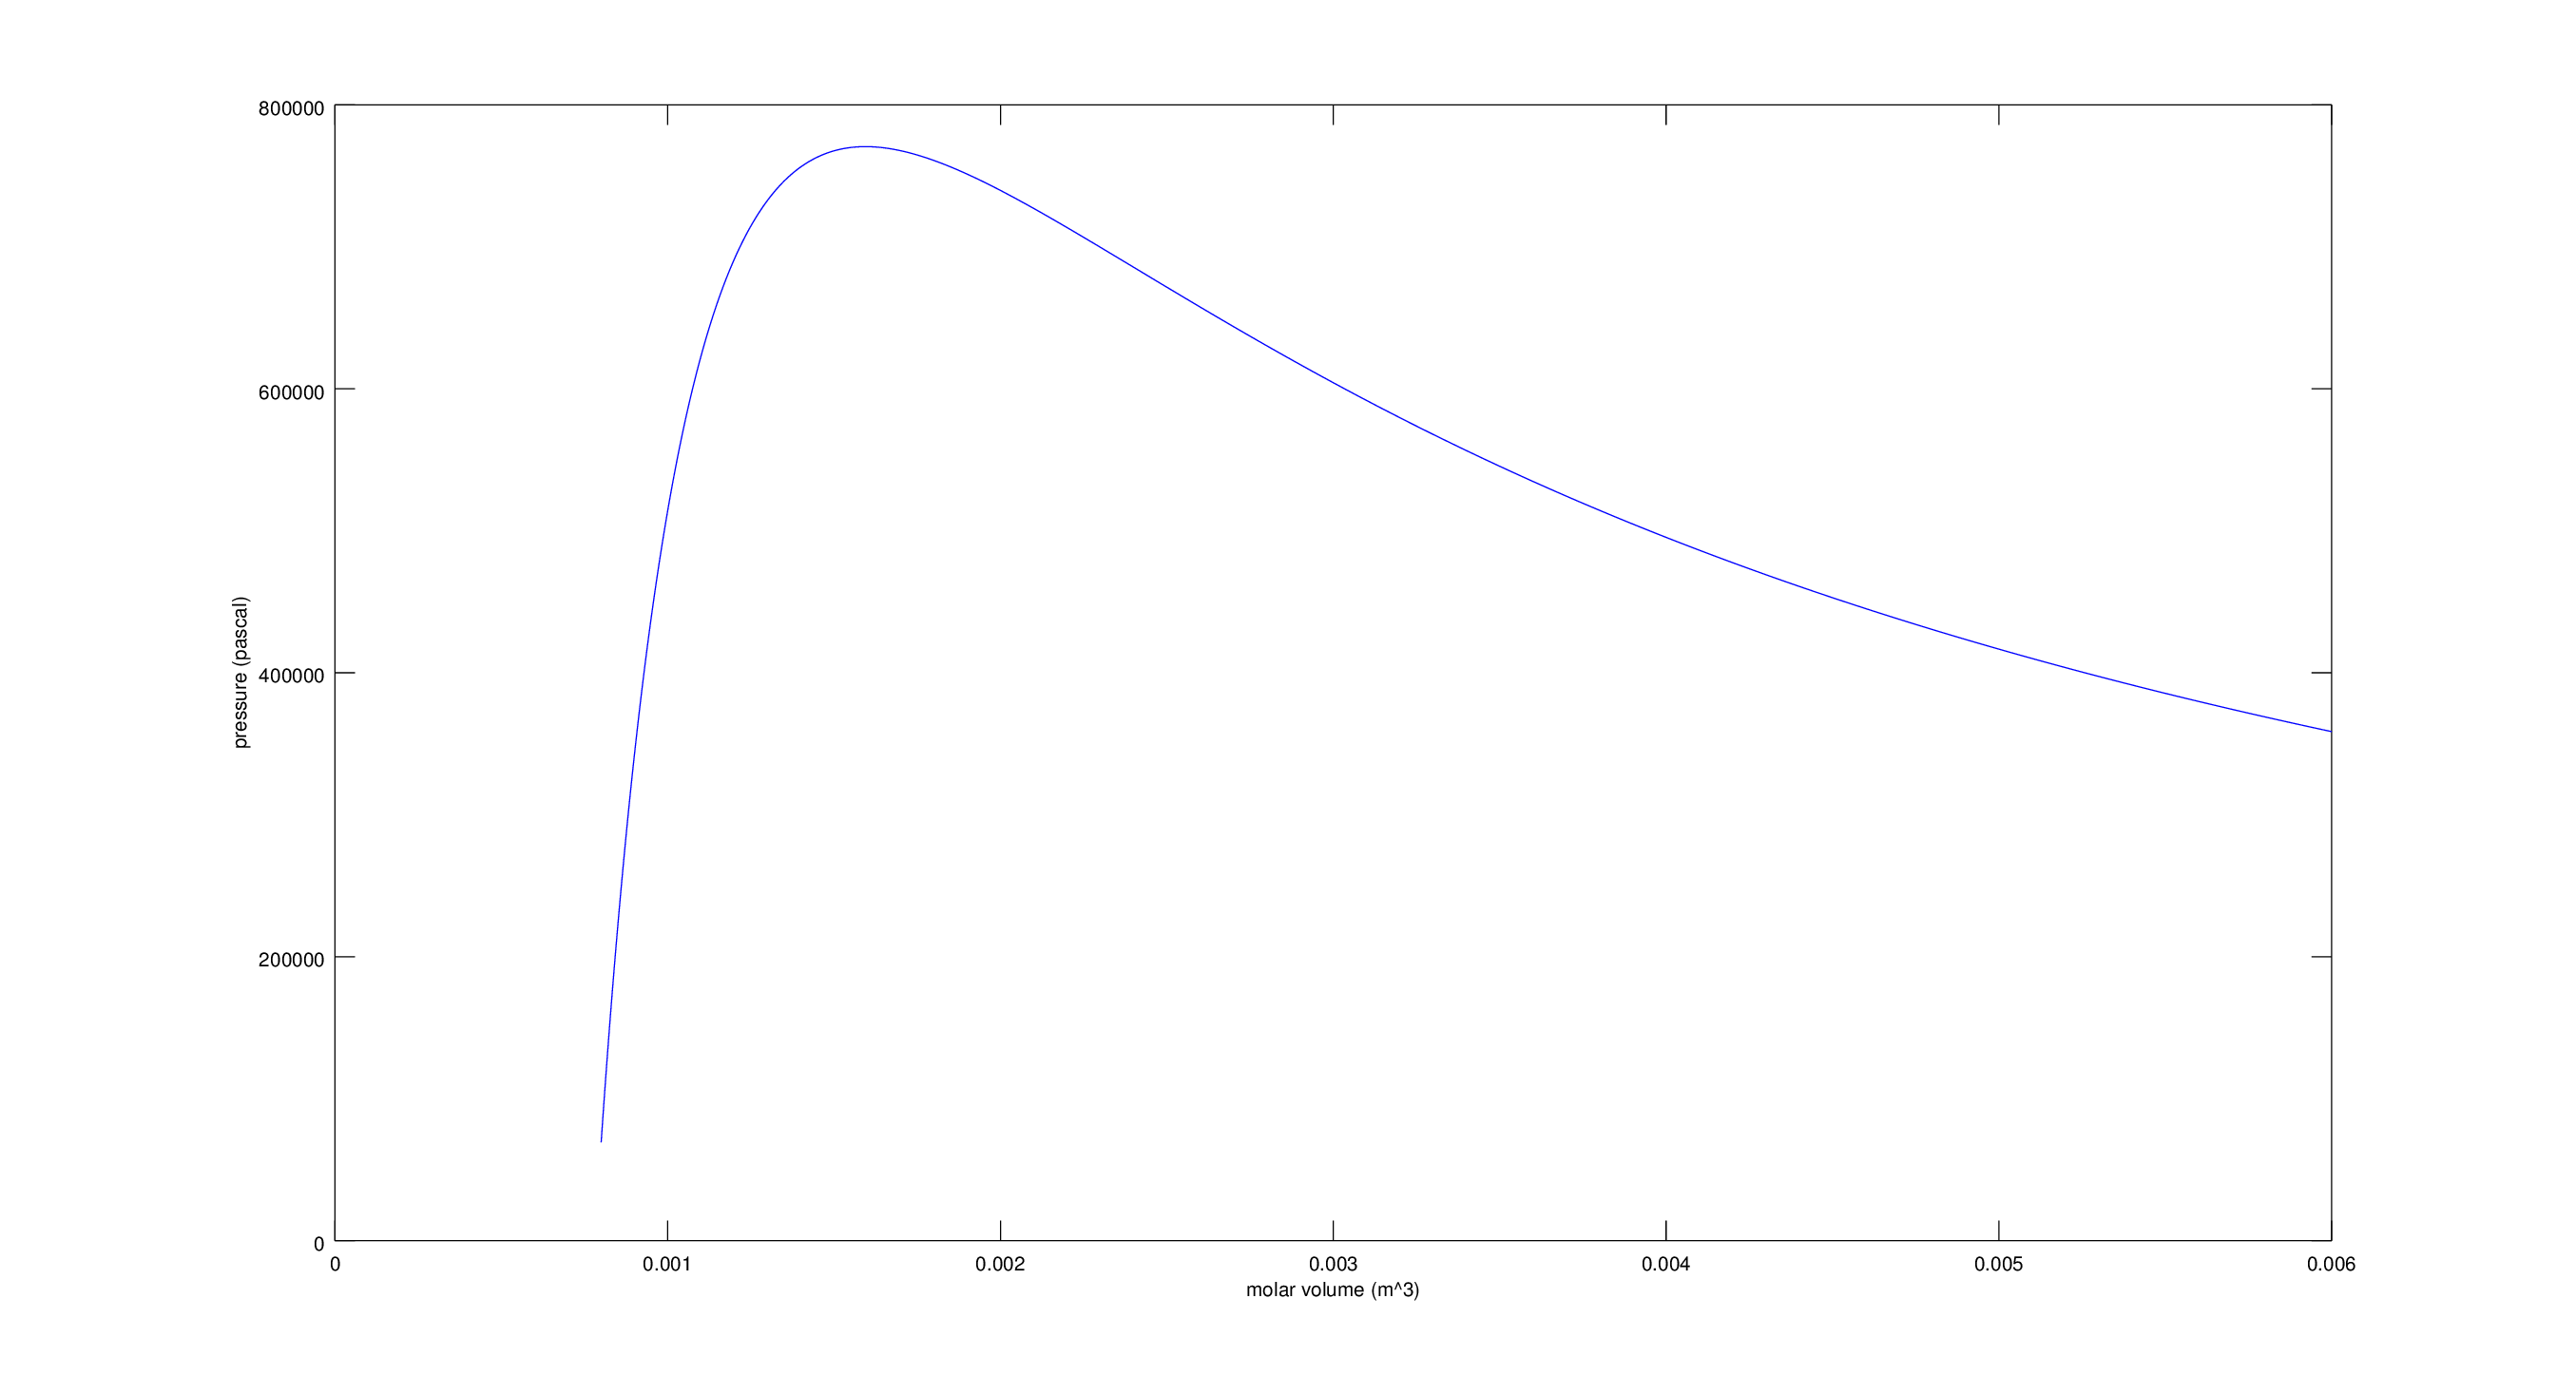
\includegraphics[scale=.35]{two}\\\\\\\\

b)  Calculate the work done to compress .3 mole of this gas from $5E-2m^3$ to $2.5E-4m^3$ at constant temperature using the van der Waals equations of state, note that \(nv=V\) where n is the number of moles and V is the volume and \(dV=ndv\).\[w=\int P(V)dV=\int_{5/3E-1}^{5/6E-3}(\frac{RT}{v-b}-\frac{a}{v^2})*.3dv=[(RT\ln(v-b)+\frac{a}{v})*.3]\mid_{5/3E-1}^{5/6E-3}=-3.24E3J\]So it takes over three thousand Jules to compress the gas using this model.  What is the result if instead we use \(P=\frac{nRT}{V}\)?\[w=\int P(V)dV=\int_{5E-2}^{2.5E-4}\frac{nRT}{V}dV=nRT\ln(V)\mid_{5E-2}^{2.5E-4}=-3.96E3J\]So using the ideal gas model we get that it takes almost four thousand Jules a significant increase in energy needed for compression.






















\end{document}